%%%%%%%%%%%%%%%%%%%%%%%%%%%%%%%%%%%%%%%%%
% Appendix
% 
% $Date$
% $Rev$:
% $Author$


\appendix

% \chapter*{Appendix}\label{appendix}
\addcontentsline{toc}{chapter}{Appendix}
\addtocontents{toc}{\protect\setcounter{tocdepth}{-1}}

\chapter{Wrapper scripts}\label{appendix:wrapperScripts}
The \dir{bin/} directory of \Kieker's binary release contains some \file{.sh}  and %
\file{.bat} scripts to invoke tools included in \file{\mainJar{}}. %
The following sections give a short description of their functionality and %
list their usage outputs as printed to the standard output stream when %
called without command-line parameters. %
In addition to the standard output stream, the file \file{kieker.log} %
is used for logging output during execution.

% generated by the script gen-bin-usage-tex.sh with manual adjustments

\section{Script \file{convertLoggingTimestamp.sh|bat}}

The script converts \KiekerMonitoringPart{} logging timestamps, %
representing the number of nanoseconds since 1~Jan 1970 00:00 UTC, to a %
human-readable textual representation. %

\

\noindent Main-class: {\small \class{kieker.tools.loggingTimestampConverter.LoggingTimestampConverterTool}}

\paragraph*{Usage}\

\setTextListing
\lstinputlisting[caption=]{Appendix-usage-convertLoggingTimestamp.sh.inc}

\paragraph*{Example}\

\setTextListing
\begin{lstlisting}
$\lstshellprompt{}$ $\textbf{bin/convertLoggingTimestamp.sh}$ $\textbf{-\,-timestamps}$ 1283156545581511026 1283156546127117246 
1283156545581511026: Mo, 30 Aug 2010 08:22:25 +0000 (UTC) (Mo, 30 Aug 2010 10:22:25 +0200 (local time))
1283156546127117246: Mo, 30 Aug 2010 08:22:26 +0000 (UTC) (Mo, 30 Aug 2010 10:22:26 +0200 (local time))
\end{lstlisting}

\section{Script \file{logReplay.sh|bat}}

Replays filesystem monitoring logs created by \KiekerMonitoringPart{}. %
Example applications are:
\begin{compactitem}
\item Merging multiple directories containing monitoring data into a single %
output directory. 
\item Importing a filesystem monitoring log to another monitoring log, e.g., %
a database. Therefore, an appropriate \KiekerMonitoringPart{} configuration %
file must be passed to the script (see Section~\ref{sec:monitoring:configuration}).
\item Replaying a recorded filesystem monitoring log in real-time in order to simulate %
incoming monitoring data from a running system, e.g., via JMS~(see also Appendix~\ref{appendix:usingJMS}). 
\end{compactitem}

\

\noindent Main-class: {\small \class{kieker.tools.logReplayer.FilesystemLogReplayerStarter}}

\paragraph*{Usage}\

\setTextListing
\lstinputlisting[caption=]{Appendix-usage-logReplay.sh.inc}

\paragraph*{Example}\

\noindent The following command replays the monitoring testdata included in %
the binary release to another directory:

\setTextListing
\begin{lstlisting}
$\lstshellprompt{}$ $\textbf{bin/logReplay.sh}$
  $\textbf{-\,-inputdirs}$ $\distributedTestdataDirDistro$ 
  $\textbf{-\,-keep-logging-timestamps}$ $true$ 
  $\textbf{-\,-realtime}$ $false$
\end{lstlisting}

\section{Script \file{trace-analysis.sh|bat}}

Calls \KiekerTraceAnalysis{} to analyze and visualize monitored trace data, %
as described in Chapter~\ref{chap:aspectJ}.

\

\noindent Main-class: {\small \class{kieker.tools.traceAnalysis.TraceAnalysisTool}}

\paragraph*{Usage}\

\setTextListing
\lstinputlisting[caption=]{Appendix-usage-trace-analysis.sh.inc}

\paragraph*{Example}\

\noindent The following commands generate a deployment-level operation dependency 
graph and convert it to pdf format:

\setTextListing
\begin{lstlisting}
$\lstshellprompt{}$ $\textbf{bin/trace-analysis.sh}$
  $\textbf{-\,-inputdirs}$ $\distributedTestdataDirDistro$ 
  $\textbf{-\,-outputdir}$ . 
  $\textbf{-\,-plot-Deployment-Operation-Dependency-Graph}$
$\lstshellprompt{}$ $\textbf{dot}$ $\textbf{-T}$ pdf
  deploymentOperationDependencyGraph.dot > deploymentOperationDependencyGraph.pdf
\end{lstlisting}

\noindent Additional examples can be found in Chapter~\ref{chap:aspectJ} and %
Appendix~\ref{appendix:traceAnalysisOutputExamples}.

\section{Script \file{dotPic-fileConverter.sh|bat}}

Converts each \file{.dot} and \file{.pic} file, e.g., diagrams generated by %
\KiekerTraceAnalysis{} (Section\ref{chap:aspectJ}), located in a directory %
into desired grahpic output formats. %
This scripts simply calls the \textit{graphviz} and \textit{plotutils} tools \file{dot} and \file{pic2plot}.

\paragraph*{Usage}\

\setTextListing
\lstinputlisting[caption=,firstline=3,lastline=3]{Appendix-usage-dotPic-fileConverter.sh.inc}

\paragraph*{Example}\

\noindent The following command converts each \file{.dot} and \file{.pic} file located in the %
directory \dir{out/} to files in \file{.pdf} and \file{.png} format:

\setTextListing
\begin{lstlisting}
$\lstshellprompt{}$ $\textbf{bin/dotPic-fileConverter.sh}$ out/ pdf png
\end{lstlisting}

\chapter{\KiekerMonitoringPart{} Default Configuration}\label{sec:appdx:monitoringproperties}
This is the file \file{\monitoringPropertiesFile} from the binary release and 
constitutes \KiekerMonitoringPart{}'s default configuration. %
Section~\ref{sec:monitoring:configuration} describes how to use a custom configuration.

\

\setPropertiesListing
\lstinputlisting[caption=\monitoringPropertiesFile]{../../META-INF/kieker.monitoring.properties}


\chapter{Additional Source Code Listings}\label{appendix:additionalSourceCode}
\section{MyNamedPipeManager and MyPipe}\label{appendix:pipeListings}

\enlargethispage{1cm}

      \setJavaCodeListing
      \lstinputlisting[firstline=22, firstnumber=22,caption=MyNamedPipeManager.java]{\customComponentsBookstoreApplicationDir/src/kicker/examples/userguide/ch3and4bookstore/MyNamedPipeManager.java}
\newpage
      \setJavaCodeListing
      \lstinputlisting[firstline=22, firstnumber=22, caption=MyPipe.java]{\customComponentsBookstoreApplicationDir/src/kicker/examples/userguide/ch3and4bookstore/MyPipe.java}
      
      \setJavaCodeListing
      \lstinputlisting[firstline=21, firstnumber=21, caption=PipeData.java]{\customComponentsBookstoreApplicationDir/src/kicker/examples/userguide/ch3and4bookstore/PipeData.java}

\chapter{Example Console Outputs}\label{appendix:exampleConsoleOutputs}
\section{Quick Start Example (Chapter~\ref{chap:example})}\label{sec:appendix:manualInstrumentation:output}
% \subsubsection{Monitoring}
% 		The following listing shows the produced log during a run of the Bookstore Application with the manual monitoring probes.
\setTextListing
\begin{lstlisting}[caption=Execution of the manually instrumented Bookstore application (Section~\ref{sec:example:monitoring})]
Apr 28, 2011 5:15:25 PM kieker.monitoring.core.configuration.Configuration createSingletonConfiguration
INFO: Loading properties from properties file in classpath: 'META-INF/kieker.monitoring.properties'
Apr 28, 2011 5:15:25 PM kieker.monitoring.core.configuration.Configuration loadConfigurationFromResource
WARNING: File 'META-INF/kieker.monitoring.properties' not found in classpath
Apr 28, 2011 5:15:25 PM kieker.monitoring.core.controller.MonitoringController createInstance
INFO: Current State of kieker.monitoring (1.3-20110427) Status: 'enabled'
	Name: 'KIEKER-SINGLETON'; Hostname: 'Kaapstad'; experimentID: '1'
WriterController:
	Number of Inserts: '0'
	Automatic assignment of logging timestamps: 'true'
Writer: 'kieker.monitoring.writer.filesystem.AsyncFsWriter'
	Configuration:
		kieker.monitoring.writer.filesystem.AsyncFsWriter.QueueFullBehavior='0'
		kieker.monitoring.writer.filesystem.AsyncFsWriter.QueueSize='10000'
		kieker.monitoring.writer.filesystem.AsyncFsWriter.customStoragePath=''
		kieker.monitoring.writer.filesystem.AsyncFsWriter.storeInJavaIoTmpdir='true'
	Writer Threads (1): 
		Finished: 'false'; Writing to Directory: '/tmp/kieker-20110428-151525684-UTC-Kaapstad-KIEKER-SINGLETON'
Sampling Controller: Periodic Sensor available: Current Poolsize: '0'; Scheduled Tasks: '0'
Bookstore.main: Starting request 0
Bookstore.main: Starting request 1
Apr 28, 2011 5:15:25 PM kieker.monitoring.writer.filesystem.MappingFileWriter writeMapping
INFO: Registered monitoring record type with id '1':kieker.common.record.OperationExecutionRecord
Bookstore.main: Starting request 2
Bookstore.main: Starting request 3
Bookstore.main: Starting request 4
\end{lstlisting}

\newpage
% \subsubsection{Analysis}
% 		The second listing is the log during the analysis of the produced data. It can be seen that some of the calls are accepted and some others refused.
\setTextListing
\begin{lstlisting}[caption=Execution of the example analysis (Section~\ref{sec:example:analysis})]
19.08.2010 13:19:55 kieker.analysis.AnalysisController registerPlugin
INFO: Registered plugin bookstoreApplication.Consumer@6ac2a132
19.08.2010 13:19:55 kieker.analysis.AnalysisController registerPlugin
INFO: Plugin bookstoreApplication.Consumer@6ac2a132 also registered as record consumer
19.08.2010 13:19:55 kieker.analysis.reader.filesystem.FSDirectoryReader processInputFile
INFO: < Loading C:\Temp\tpmon-20100814-103954167-UTC\tpmon-20100814-103954184-UTC-Thread-2.dat
19.08.2010 13:19:55 kieker.common.record.MonitoringRecordTypeRegistry registerRecordTypeIdMapping
INFO: Registered record type mapping 1/kieker.common.record.OperationExecutionRecord
maximal response time exceeded by 11382559 ns: bookstoreApplication.Catalog.getBook()
maximal response time exceeded by 11251720 ns: bookstoreApplication.Catalog.getBook()
maximal response time exceeded by 80320 ns: bookstoreApplication.Catalog.getBook()
maximal response time exceeded by 27400 ns: bookstoreApplication.Catalog.getBook()
maximal response time exceeded by 81760 ns: bookstoreApplication.Catalog.getBook()
maximal response time exceeded by 24240 ns: bookstoreApplication.Catalog.getBook()
maximal response time exceeded by 82480 ns: bookstoreApplication.Catalog.getBook()
response time accepted: bookstoreApplication.Catalog.getBook()
response time accepted: bookstoreApplication.Catalog.getBook()
response time accepted: bookstoreApplication.Catalog.getBook()
14.08.2010 12:41:02 kieker.analysis.reader.filesystem.FSReader$\$$FSReaderCons execute
INFO: All reader threads provided FS_READER_TERMINATION_MARKER
\end{lstlisting}
\newpage	
\section{Trace Monitoring, Analysis \& Visualization (Chapter \ref{chap:aspectJ})}%
\label{sec:appendix:exampleConsoleOutputs:aspectJExample}
\setTextListing
\begin{lstlisting}[caption=Execution of the Bookstore with AspectJ trace instrumentation (Section~\ref{sec:traceAnalysis:instr:AspectJ})]
Bookstore.main: Starting request 0
Apr 28, 2011 4:28:29 PM kieker.monitoring.core.configuration.Configuration createSingletonConfiguration
INFO: Loading properties from properties file in classpath: 'META-INF/kieker.monitoring.properties'
Apr 28, 2011 4:28:29 PM kieker.monitoring.core.controller.MonitoringController createInstance
INFO: Current State of kieker.monitoring (1.3-20110427) Status: 'enabled'
	Name: 'KIEKER'; Hostname: 'Kaapstad'; experimentID: '1'
WriterController:
	Number of Inserts: '0'
	Automatic assignment of logging timestamps: 'true'
Writer: 'kieker.monitoring.writer.filesystem.AsyncFsWriter'
	Configuration:
		kieker.monitoring.writer.filesystem.AsyncFsWriter.QueueFullBehavior='0'
		kieker.monitoring.writer.filesystem.AsyncFsWriter.QueueSize='10000'
		kieker.monitoring.writer.filesystem.AsyncFsWriter.customStoragePath=''
		kieker.monitoring.writer.filesystem.AsyncFsWriter.storeInJavaIoTmpdir='true'
	Writer Threads (1): 
		Finished: 'false'; Writing to Directory: '/tmp/kieker-20110428-142829399-UTC-Kaapstad-KIEKER'
Sampling Controller: Periodic Sensor available: Current Poolsize: '0'; Scheduled Tasks: '0'
Apr 28, 2011 4:28:29 PM kieker.monitoring.core.registry.ControlFlowRegistry <init>
INFO: First threadId will be 7752665283541598209
Apr 28, 2011 4:28:29 PM kieker.monitoring.writer.filesystem.MappingFileWriter writeMapping
INFO: Registered monitoring record type with id '1':kieker.common.record.OperationExecutionRecord
\end{lstlisting}




\chapter{Ant Scripts}\label{appendix:antScripts}
\section{Quick Start Example (Chapter \ref{chap:example})}
The following \file{build.xml} and \file{build.properties} files can be %
used for compiling and executing the manually instrumentated Bookstore %
application and the analysis, as described in Chapter~\ref{chap:example}. %
The files are included in the directory \file{\manualInstrumentedBookstoreApplicationDirDistro{}/}.

      In order to run the analysis of the application, it is necessary to pass the location of the monitoring log directory. This is done via the parameter \textit{analysis.directory}, e.g.:
      \setBashListing
      \begin{lstlisting}[caption=Command to compile and run the instrumented Bookstore via ant]
#\lstshellprompt{}# ant run-analysis -Danalysis.directory /tmp/kicker-20120402-163314855-UTC-myHost-KIEKER-SINGLETON
\end{lstlisting}%-KIEKER


% \enlargethispage{1.2cm}
      \setXMLListing
      \lstinputlisting[caption=build.properties]{\manualInstrumentedBookstoreApplicationDir/build.properties}
      \lstinputlisting[caption=build.xml]{\manualInstrumentedBookstoreApplicationDir/build.xml}
\newpage
\section{Custom Components (Chapters \ref{chap:componentsMonitoring} and \ref{chap:componentsAnalysis})}
      The following \file{build.xml} and \file{build.properties} files can be used for compiling and executing the manually instrumentated Bookstore application with the custom components, as described in Chapters~\ref{chap:componentsMonitoring} and \ref{chap:componentsAnalysis}. %
The files are included in the directory \file{\customComponentsBookstoreApplicationDirDistro{}/}.
      \setXMLListing
      \lstinputlisting[caption=build.properties]{\customComponentsBookstoreApplicationDir/build.properties}
      \lstinputlisting[caption=build.xml]{\customComponentsBookstoreApplicationDir/build.xml}
\newpage
\section{AspectJ-based Trace Monitoring (Chapter \ref{chap:aspectJ})}
      The following \file{build.xml} and \file{build.properties} files can be used for compiling and executing the Bookstore application instrumentated with AspectJ, as described in Chapter~\ref{chap:aspectJ}. %

The files are included in the directory \file{\aspectJBookstoreApplicationDirDistro{}/}.
      \setXMLListing
      \lstinputlisting[caption=build.properties]{\aspectJBookstoreApplicationDir/build.properties}     
      \lstinputlisting[caption=build.xml]{\aspectJBookstoreApplicationDir/build.xml}

\chapter{Java~EE Servlet Container Example}\label{appendix:JavaEEServletExample}
The \Kieker{} download site\footnote{\KiekerDownloadURL{}} includes an additional %
example \file{\JavaEEServletExampleName}. Using the sample Java Web application %
iBATIS JPetStore\footnote{\url{http://ibatis.apache.org/}}, this example %
demonstrates how to employ \KiekerMonitoringPart{} for monitoring a Java application %
running in a Java~EE container---in this case, Apache Tomcat\footnote{\url{http://tomcat.apache.org/}}. %
Monitoring probes based on the Java~EE Servlet API %
and AspectJ are used to monitor execution, trace, and session data (see Section~\ref{chap:aspectJ}).

\

\WARNBOX{The example is currently only prepared for \UnixLikeSystems. However, %
based on the descriptions below, it shouldn't be too difficult to run it under %
Windows}

\section{Preparation of the Tomcat Servlet Container}

\begin{compactenum}
\item Copy the files \file{\mainJar}, \file{\commonsLoggingJar}, and \file{\aspectJWeaverJar} from %
\Kieker{}'s binary distribution to the Tomcat's \dir{lib/} directory.
\item Copy the file \file{\servletWar} from \Kieker{}'s %
binary distribution to the Tomcat's \dir{webapps/} directory.
\item Tomcat's \dir{lib/} directory contains the files \file{kieker.monitoring.properties} %
and \file{aop.xml} --- the configuration of \KiekerMonitoringPart{} and the %
AspectJ-based instrumentation. %
\item Tomcat's \file{bin/catalina.sh} file was modified to add the location %
of the \file{kieker.\-moni\-toring.properties} and the AspectJ agent to the argument %
list of the JVM call:
\end{compactenum}

\setPropertiesListing
\lstinputlisting[firstline=73,firstnumber=73,lastline=74,caption={Excerpt from catalina.sh},numbers=left]{\JavaEEServletExampleDir/Tomcat6.0.18WithJpetStore-withInstrumentedJPetStore/bin/catalina.sh}

\begin{compactenum}\setcounter{enumi}{4}
\item  A prepared \file{jpetstore.war} file is already located in the %
   Tomcat's \dir{webapps/} directory. If you want to rebuild the sources, %
   for example to modify the instrumentation, see Section~\ref{sec:Appendix:JPetStoreExample:rebuild}. 
\end{compactenum}


\section{JPetStore and \KiekerMonitoringPart{} Control Servlet}

\noindent We will now start the Tomcat server and generate some monitoring data by manually %
accessing the JPetStore web application. 

\

\enlargethispage{1.5cm}

\begin{compactenum}
\item Start the Tomcat server using the \file{bin/startup.sh} script in the 
   Tomcat's \dir{bin/} directory (you may have to execute "\texttt{chmod +x bin/*.sh}" %
   in order to set the executable flags of the shell scripts). %
   You should make sure, that the Tomcat started properly, by taking 
   a look at the \file{logs/catalina.out} file. %
   On error, the file \file{logs/localhost.<date>.log} may contain details % 
   to resolve the issue.
\item Now, you can access the JPetStore application by opening the URL
   \url{http://localhost:8080/jpetstore/} (Figure~\ref{fig:jpetstore}). %
   \Kieker{} intialization messages should appear in \file{logs/catalina.out}. %
   The output includes the information where the monitoring data is written to
   (should be Tomcat's \dir{temp/tpmon-<DATE-TIME>/} directory).
\item  Browse through the application to generate some monitoring data. %
   This data can be analyzed and visualized using \KiekerTraceAnalysis{}, %
   as described in Chapter~\ref{chap:aspectJ}.
\item \Kieker{} includes a servlet to control the status of \KiekerMonitoringPart{}. %
   It can be accessed via \url{http://localhost:8080/kieker-monitoring-servlet-\version/} %
   (Figure~\ref{fig:controlServlet}).
\end{compactenum}

\begin{figure}[h]\centering
\hfill
\subfigure[iBATIS JPetStore]{\label{fig:jpetstore}%
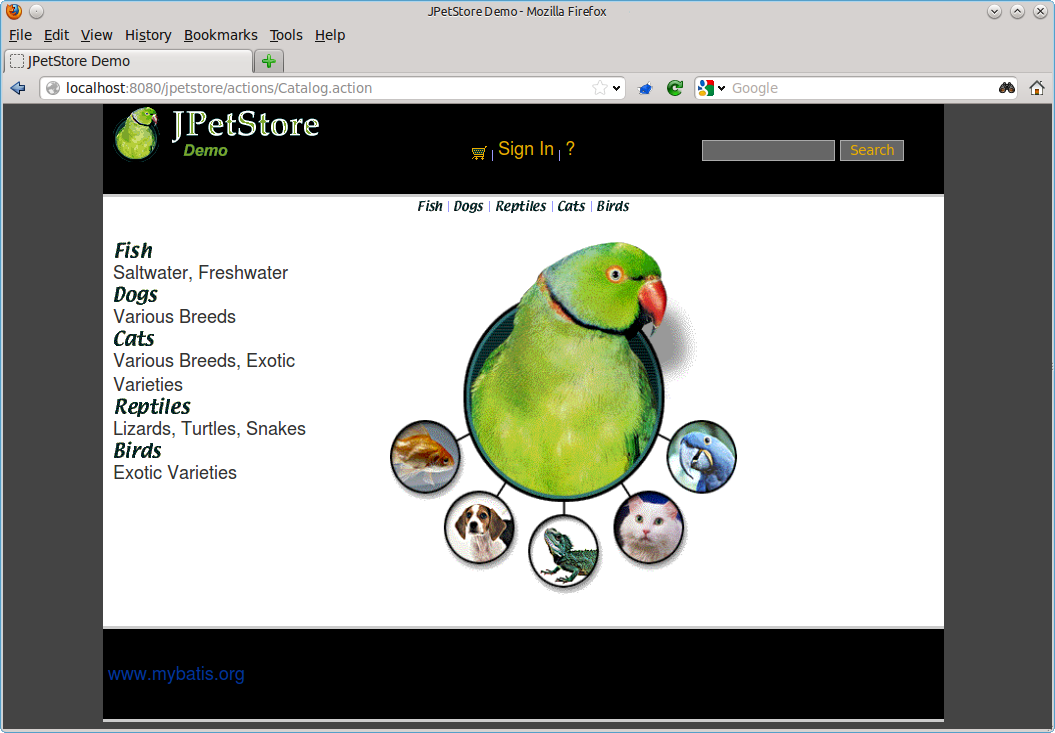
\includegraphics[width=0.45\textwidth]{images/jpetstore-example-FFscrsh}}
\hfill
\subfigure[\KiekerMonitoringPart{} control servlet]{\label{fig:controlServlet}%
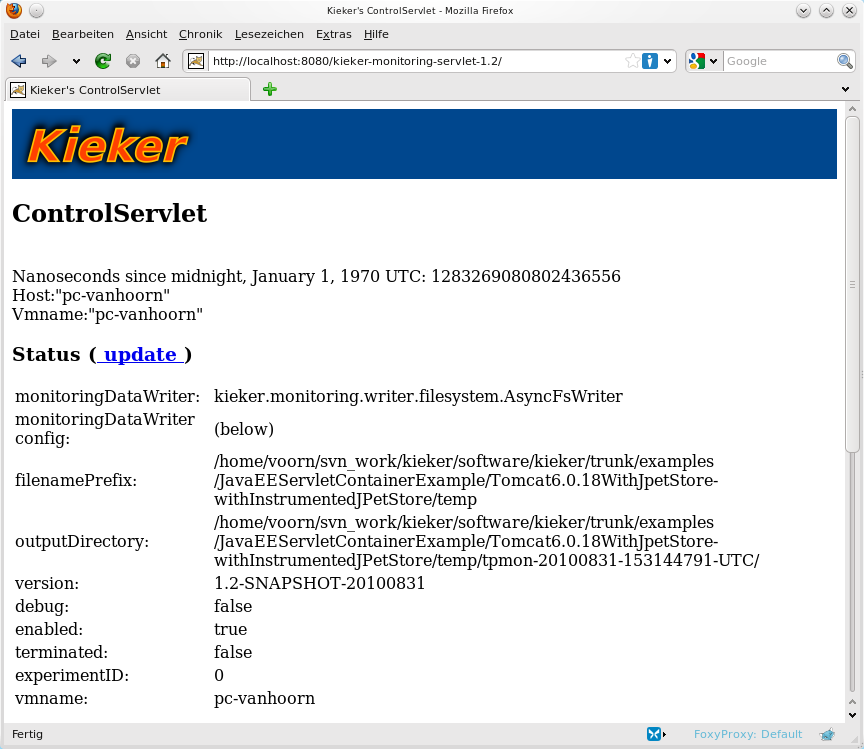
\includegraphics[width=0.45\textwidth]{images/kieker-servlet-FFscrsh}}
\hfill
\caption{}
\end{figure}

\newpage

\section{Rebuilding the JPetStore Application}\label{sec:Appendix:JPetStoreExample:rebuild}

\noindent In order to rebuild the JPetStore sources (located in \dir{JPetStore-5.0-instrumented/}), 
the following steps are required:

\

\begin{compactenum}
\item Copy the \file{\mainJar{}} from \Kieker{}'s
   binary distribution to the JPetStore's \dir{devlib/} directory. %
   It is required for the annotation-based instrumentation %
   (\texttt{@Ope\-rationExecutionMonitoringProbe}), as described in Chapter~\ref{chap:aspectJ}
\item Build the JPetStore with the \file{build.xml} by calling \texttt{ant} from %
    within \dir{build/} directory. 
\item You'll find the packaged JPetStore \file{.war}-file in \dir{build/wars/}.
\item Copy the file to the Tomcat's \dir{webapps/} directory.
\end{compactenum}



\chapter{Using the JMS Writer and Reader}\label{appendix:usingJMS}
This chapter gives a brief description on how to use the \class{AsyncJMSWriter} and \class{JMSReader} %
classes. The directory \dir{\JMSBookstoreApplicationDirDistro/} contains the %
sources, ant scripts etc.\ used in this example. It is based on the Bookstore %
application with manual instrumentation presented in Chapter~\ref{chap:example}. %

The following sections provide step-by-step instructions for the %
JMS server implementations ActiveMQ (Section~\ref{example:jms:activemq}), %
HornetQ~(\ref{example:jms:hornetq}), and OpenJMS~(\ref{example:jms:openjms}).
The general procedure for each example is the following:

\medskip

\begin{compactenum}
 \item Download and prepare the respective JMS server implementation
 \item Copy required libraries to the example directory
 \item Start the JMS server
 \item Start the analysis instance which receives records via JMS
 \item Start the monitoring instance which sends records via JMS
\end{compactenum}

\

\WARNBOX{Due to a bug in the JMS-server some executions of the following examples could be problematic if paths with space characters are used. Try to avoid such paths.}

\section{ActiveMQ}\label{example:jms:activemq}

\subsection{Download and Prepare ActiveMQ}

Download an ActiveMQ archive from \url{http://activemq.apache.org/download.html}
and decompress it to the base directory of the example. Note, that there are two different %
distributions, one for Unix/Linux/Cygwin and another one for Windows. 

Under \UnixLikeSystems{}, you'll need to set the executable-bit of the start script:

\setBashListing
\begin{lstlisting}[caption=]
 #\lstshellprompt{}# chmod +x bin/activemq
\end{lstlisting}

\noindent Also under \UnixLikeSystems{}, make sure that the file \file{bin/activemq} %
includes UNIX line endings (e.g., using your favorite editor or the \textit{dos2unix} tool).

\subsection{Copy Kieker and ActiveMQ Libraries}

\paragraph*{Kieker Libraries}

Copy the following file from Kieker's binary distribution to %
the example's \dir{lib/} directory.

\enlargethispage{0.5cm}
\medskip

\begin{compactenum}
 \item \file{\mainJarEMF} (from \dir{dist/})
\end{compactenum}

\paragraph*{ActiveMQ Libraries}

Copy the following files from the ActiveMQ release to the %
\dir{lib/} directory of this example:

\medskip

\begin{compactenum}
\item \file{activemq-all-<version>.jar} (from ActiveMQ's base directory)
\item \file{slf4j-log4j<version>.jar} (from ActiveMQ's \dir{lib/optional} directory)
\item \file{log4j-<version>.jar} (from ActiveMQ's \dir{lib/optional} directory)
\end{compactenum}

\subsection{Kieker Monitoring Configuration for ActiveMQ}

The file \file{\JMSBookstoreApplicationDirDistro/META-INF/kieker.monitoring.\-pro\-perties-activeMQ} %
is already configured to use the \class{AsyncJMSWriter} via ActiveMQ. The important properties are %
the definition of the provider URL and the context factory:

\setPropertiesListing
\lstinputlisting[firstline=143,lastline=143,caption=Excerpt from \file{kieker.monitoring.properties-activemq} configuring the provider URL of the JMS writer via ActiveMQ]{\JMSBookstoreApplicationDir/META-INF/kieker.monitoring.properties-activemq}

\setPropertiesListing
\lstinputlisting[firstline=152,lastline=152,caption=Excerpt from \file{kieker.monitoring.properties-activemq} configuring the connection factory of the JMS writer via ActiveMQ]{\JMSBookstoreApplicationDir/META-INF/kieker.monitoring.properties-activemq}

\subsection{Running the Example}

% \paragraph*{Execution}%
 The execution of the example is performed by the following three steps:
\begin{enumerate}
\item Start the JMS server (you may have to set your \class{JAVA\_HOME} variable first):

\setBashListing
\begin{lstlisting}[caption=Start of the JMS server under UNIX-like systems]
#\lstshellprompt{}# bin/activemq start
\end{lstlisting}
\begin{lstlisting}[caption=Start of the JMS server under Windows]
#\lstshellprompt{}# bin\#activemq
\end{lstlisting}
\item Start the analysis part (in a new terminal):
\setBashListing
\begin{lstlisting}[caption=]
#\lstshellprompt{}# ant run-analysis-activemq
\end{lstlisting}
\item Start the instrumented Bookstore (in a new terminal):
\setBashListing
\begin{lstlisting}[caption=]
#\lstshellprompt{}# ant run-monitoring-activemq
\end{lstlisting}
\end{enumerate}


\section{HornetQ}\label{example:jms:hornetq}

\subsection{Download and Prepare HornetQ}

Download a HornetQ archive from \url{http://www.jboss.org/hornetq/downloads.html} %
and decompress it to the root directory of the example. 

\noindent You need to create a queue in the HornetQ configuration file %
\file{config/stand-alone/non-clustered/hornetq-jms.xml}, as shown in Listing~\ref{lst:hornetq:config:queue}.

\setXMLListing
\begin{lstlisting}[caption=Queue definition to be added to the HornetQ configuration file,label=lst:hornetq:config:queue,numbers=none]
  <queue name="queue1">
      <entry name="/queue/queue1"/>
  </queue>
\end{lstlisting}

\subsection{Copy Kieker and HornetQ Libraries}

\paragraph*{Kieker Libraries}

Copy the following file from Kieker's binary distribution to %
the example's \dir{lib/} directory.

\medskip

\begin{compactenum}
 \item \file{\mainJarEMF} (from \dir{dist/})
\end{compactenum}

\paragraph*{HornetQ Libraries}

Copy the following files from the HornetQ \dir{lib/} folder to the %
\dir{lib/} directory of this example:

\medskip

\begin{compactenum}
\item \file{hornetq-jms-client.jar}
\item \file{hornetq-core-client.jar}
\item \file{jboss-jms-api.jar}
\item \file{jnp-client.jar}
\item \file{netty.jar}
\end{compactenum}

\subsection{Kieker Monitoring Configuration for HornetQ}

The file \file{\JMSBookstoreApplicationDirDistro/META-INF/kieker.monitoring.\-pro\-perties-hornetq} %
is already configured to use the \class{AsyncJMSWriter} via HornetQ. The important properties are %
the definition of the provider URL, the context factory, and the queue:

\setPropertiesListing
\lstinputlisting[firstline=143,lastline=143,caption=Excerpt from \file{kieker.monitoring.properties-hornetq} configuring the provider URL of the JMS writer via HornetQ]{\JMSBookstoreApplicationDir/META-INF/kieker.monitoring.properties-hornetq}

\setPropertiesListing
\lstinputlisting[firstline=152,lastline=152,caption=Excerpt from \file{kieker.monitoring.properties-hornetq} configuring the connection factory of the JMS writer via HornetQ]{\JMSBookstoreApplicationDir/META-INF/kieker.monitoring.properties-hornetq}

\subsection{Running the Example}

% \paragraph*{Execution}%
 The execution of the example is performed by the following three steps:
\begin{enumerate}
\item Start the JMS server:

\setBashListing
\begin{lstlisting}[caption=Start of the JMS server under UNIX-like systems]
#\lstshellprompt{}# ./run.sh
\end{lstlisting}
\begin{lstlisting}[caption=Start of the JMS server under Windows]
#\lstshellprompt{}# run.bat
\end{lstlisting}

Note that the script must be called from within HornetQ's \dir{bin/} directory.

\item Start the analysis part (in a new terminal):
\setBashListing
\begin{lstlisting}[caption=]
#\lstshellprompt{}# ant run-analysis-hornetq
\end{lstlisting}
\item Start the instrumented Bookstore (in a new terminal):
\setBashListing
\begin{lstlisting}[caption=]
#\lstshellprompt{}# ant run-monitoring-hornetq
\end{lstlisting}
\end{enumerate}

\section{OpenJMS}\label{example:jms:openjms}

\subsection{Download and Prepare OpenJMS}

Download an OpenJMS install archive from \url{http://openjms.sourceforge.net} %
and decompress it to the root directory of the example. Under UNIX-like systems, make sure that the executable-bit of all scripts within the \dir{bin/} directory are set.

\subsection{Copy Kieker and OpenJMS Libraries}

\paragraph*{Kieker Libraries}

Copy the following files from Kieker's binary distribution to %
the example's \dir{lib/} directory.

\medskip

\begin{compactenum}
 \item \file{\mainJarEMF} (from \dir{dist/})
 \item \file{\commonsLoggingJar} (from \dir{lib/})
\end{compactenum}

\paragraph*{OpenJMS Libraries}

Copy the following files from the OpenJMS \dir{lib/} folder to the %
\dir{lib/} directory of this example:

\medskip

\begin{compactenum}
\item \file{openjms-<version>.jar}
\item \file{openjms-common-<version>.jar}
\item \file{openjms-net-<version>.jar}
\item \file{jms-<version>.jar}
\item \file{concurrent-<version>.jar}
\item \file{spice-jndikit-<version>.jar}
\end{compactenum}

\subsection{Kieker Monitoring Configuration for OpenJMS}

The file \file{\JMSBookstoreApplicationDirDistro/META-INF/kieker.monitoring.\-pro\-perties-openjms} %
is already configured to use the \class{AsyncJMSWriter} via OpenJMS. The important properties are %
the definition of the provider URL and the context factory:

\setPropertiesListing
\lstinputlisting[firstline=143,lastline=143,caption=Excerpt from \file{kieker.monitoring.properties-openjms} configuring the provider URL of the JMS writer via OpenJMS]{\JMSBookstoreApplicationDir/META-INF/kieker.monitoring.properties-openjms}

\setPropertiesListing
\lstinputlisting[firstline=152,lastline=152,caption=Excerpt from \file{kieker.monitoring.properties-openjms} configuring the connection factory of the JMS writer via OpenJMS]{\JMSBookstoreApplicationDir/META-INF/kieker.monitoring.properties-openjms}

\subsection{Running the Example}

% \paragraph*{Execution}%
 The execution of the example is performed by the following three steps:
\begin{enumerate}
\item Start the JMS server (you may have to set your \class{JAVA\_HOME} and \class{OPENJMS\_HOME} variables first):

\setBashListing
\begin{lstlisting}[caption=Start of the JMS server under UNIX-like systems]
#\lstshellprompt{}# openjms-<version>/bin/startup.sh
\end{lstlisting}
\begin{lstlisting}[caption=Start of the JMS server under Windows]
#\lstshellprompt{}# openjms-<version>\bin\startup.bat
\end{lstlisting}
\item Start the analysis part (in a new terminal):
\setBashListing
\begin{lstlisting}[caption=]
#\lstshellprompt{}# ant run-analysis-openjms
\end{lstlisting}
\item Start the instrumented Bookstore (in a new terminal):
\setBashListing
\begin{lstlisting}[caption=]
#\lstshellprompt{}# ant run-monitoring-openjms
\end{lstlisting}
\end{enumerate}


\chapter{Sigar-Based Samplers for System-Level Monitoring}\label{appendix:SigarBasedSamplers}
This chapter gives a brief description on how to use the included %
periodic samplers (Section~\ref{sec:componentsMonitoring:monitoringController:periodicSamplers}) %
for monitoring CPU utilization and memory/swap usage. %
The directory \dir{\SigarExampleDirDistro/} contains the %
sources, ant scripts etc.\ used in this example. %
These samplers employ the Sigar API~\cite{HypericSigarWebsite}. \\%

\section{Preparation}

\begin{compactenum}
\item Copy the files \file{\mainJarEMF} and \file{\sigarJar} from the %
binary distribution to the example's \dir{lib/} directory.
\item Additionally, depending on the underlying system platform, %
corresponding Sigar native libraries need to be placed in the example's \dir{lib/} directory. %
Kieker's \dir{lib/sigar-native-libs/} folder already includes the right libraries for 32 and 64~bit Linux/Windows platforms. %
Native libraries for other platforms can be downloaded from~\cite{HypericSigarWebsite}. %
\end{compactenum}

\section{Using the Sigar-Based Samplers}

\WARNBOX{
	Using a very short sampling period with Sigar ($< 500$ ms) can result in monitoring log entries with NaN values. 
}

The Sigar API~\cite{HypericSigarWebsite} provides access to a number of system-level inventory and monitoring data, %
e.g., regarding memory, swap, cpu, file system, and network devices. %
Kieker includes Sigar-based samplers %
for monitoring CPU utilization %
(\class{CPUsDetailedPercSampler}, \class{CPUsCombinedPercSampler}) %
and memory/swap usage (\class{MemSwapUsageSampler}). %
When registered as a periodic sampler (Section~\ref{sec:componentsMonitoring:monitoringController:periodicSamplers}), %
these samplers collect the data of interest employing the Sigar API, %
and write monitoring records of types \class{CPUUtilizationRecord}, %
\class{ResourceUtilizationRecord}, and \class{MemSwapUsageRecord} respectively %
to the configured monitoring log/stream. %

Listing~\ref{listing:sigarSamplerMonitoringStarterExample} shows an excerpt from %
this example's \class{MonitoringStarter} %
which creates and registers two Sigar-based peridioc samplers. %
For reasons of performance and thread-safety, the \class{SigarSamplerFactory} %
should be used to create instances of the Sigar-based Samplers. 

%\pagebreak

\setJavaCodeListing
\lstinputlisting[firstline=38, lastline=51, firstnumber=38, caption=Excerpt from MonitoringStarter.java, label=listing:sigarSamplerMonitoringStarterExample]{\SigarExampleDir/src/kieker/examples/userguide/appendixSigar/MonitoringStarter.java}

\noindent Based on the existing samplers, users can easily create custom Sigar-based %
samplers by extending the class \class{AbstractSigarSampler}. For example, Listing~%
\ref{listing:sigarSamplerMethod} in Section~\ref{sec:componentsMonitoring:monitoringController:periodicSamplers} %
shows the \class{MemSwapUsageSampler}'s \method{sample} method. %
Typically, it is also required to define a corresponding monitoring record type, %
as explained in Section~\ref{sec:componentsMonitoring:monitoringRecords}. %
When implementing custom Sigar-based samplers, the \class{SigarSamplerFactory}'s \method{getSigar} method should %
be used to retrieve a \class{Sigar} instance. %

This example uses a stand-alone Java application to set up %
a Sigar-based monitoring process. When using servlet containers,  %
users may consider implementing this routine as a \class{ServletContextListener}, %
which are executed when the container is started and shutdown. %
As an example, Kieker includes a \class{CPUMemUsageServletContextListener}. %

\section{Executing the Example}

The execution of the example is performed by the following two steps:\\

\begin{compactenum}
\item Monitoring CPU utilization and memory usage for 30~seconds (class \class{MonitoringStarter}):
\setBashListing
\begin{lstlisting}[caption=]
#\lstshellprompt{}# #\textbf{ant}# run-monitoring
\end{lstlisting}

Kieker's console output lists the location of the directory containing the file system %
monitoring log. The following listing shows an excerpt: %

%\enlargethispage{1.5cm}
\pagebreak
\setBashListing
\begin{lstlisting}
 Writer: 'kieker.monitoring.writer.filesystem.AsyncFsWriter'
     Configuration:
             kieker.monitoring.writer.filesystem.AsyncFsWriter.QueueFullBehavior='0'
             kieker.monitoring.writer.filesystem.AsyncFsWriter.QueueSize='10000'
             kieker.monitoring.writer.filesystem.AsyncFsWriter.customStoragePath=''
             kieker.monitoring.writer.filesystem.AsyncFsWriter.storeInJavaIoTmpdir='true'
     Writer Threads (1): 
             Finished: 'false'; Writing to Directory: '/tmp/kieker-20110511-10095928-UTC-avanhoorn-thinkpad-KIEKER-SINGLETON'
\end{lstlisting}

A sample monitoring log can be found in the directory \dir{\SigarExampleDirDistro/testdata/kieker-20110511-10095928-UTC-avanhoorn-thinkpad-KIEKER-SINGLETON/}.

\item Analyzing the monitoring data (class \class{AnalysisStarter}):

\setBashListing
\begin{lstlisting}[caption=]
#\lstshellprompt{}# #\textbf{ant}# run-analysis #\textbf{-Danalysis.directory}#=</path/to/monitoring/log/>
\end{lstlisting}

You need to replace \dir{</path/to/monitoring/log/>} by the location of the file system monitoring log. %
You can also use the above-mentioned monitoring log included in the example. %

The \class{AnalysisStarter} produces a simple console output for each monitoring record, %
as shown in the following excerpt: 

\setBashListing
\begin{lstlisting}
Wed, 11 May 2011 10:10:01 +0000 (UTC): [CPU] host: thinkpad ; cpu-id: 0 ; utilization: 0.00 %
Wed, 11 May 2011 10:10:01 +0000 (UTC): [CPU] host: thinkpad ; cpu-id: 1 ; utilization: 0.00 %
Wed, 11 May 2011 10:10:01 +0000 (UTC): [Mem/Swap] host: thinkpad ; mem usage: 722.0 MB ; swap usage: 0.0 MB
Wed, 11 May 2011 10:10:06 +0000 (UTC): [CPU] host: thinkpad ; cpu-id: 0 ; utilization: 5.35 %
Wed, 11 May 2011 10:10:06 +0000 (UTC): [CPU] host: thinkpad ; cpu-id: 1 ; utilization: 1.31 %
Wed, 11 May 2011 10:10:06 +0000 (UTC): [Mem/Swap] host: thinkpad ; mem usage: 721.0 MB ; swap usage: 0.0 MB
Wed, 11 May 2011 10:10:11 +0000 (UTC): [CPU] host: thinkpad ; cpu-id: 0 ; utilization: 1.80 %
Wed, 11 May 2011 10:10:11 +0000 (UTC): [CPU] host: thinkpad ; cpu-id: 1 ; utilization: 0.20 %
Wed, 11 May 2011 10:10:11 +0000 (UTC): [Mem/Swap] host: thinkpad ; mem usage: 721.0 MB ; swap usage: 0.0 MB
Wed, 11 May 2011 10:10:16 +0000 (UTC): [CPU] host: thinkpad ; cpu-id: 0 ; utilization: 1.40 %
Wed, 11 May 2011 10:10:16 +0000 (UTC): [CPU] host: thinkpad ; cpu-id: 1 ; utilization: 0.79 %
Wed, 11 May 2011 10:10:16 +0000 (UTC): [Mem/Swap] host: thinkpad ; mem usage: 721.0 MB ; swap usage: 0.0 MB
Wed, 11 May 2011 10:10:21 +0000 (UTC): [CPU] host: thinkpad ; cpu-id: 0 ; utilization: 1.80 %
Wed, 11 May 2011 10:10:21 +0000 (UTC): [CPU] host: thinkpad ; cpu-id: 1 ; utilization: 0.79 %
Wed, 11 May 2011 10:10:21 +0000 (UTC): [Mem/Swap] host: thinkpad ; mem usage: 721.0 MB ; swap usage: 0.0 MB
Wed, 11 May 2011 10:10:26 +0000 (UTC): [CPU] host: thinkpad ; cpu-id: 0 ; utilization: 0.40 %
Wed, 11 May 2011 10:10:26 +0000 (UTC): [CPU] host: thinkpad ; cpu-id: 1 ; utilization: 0.59 %
Wed, 11 May 2011 10:10:26 +0000 (UTC): [Mem/Swap] host: thinkpad ; mem usage: 721.0 MB ; swap usage: 0.0 MB
\end{lstlisting}


\end{compactenum}


\chapter{Libraries}\label{appendix:libraries}
    The following table shows all libraries which are used by \Kieker\ and explains them briefly. %
These libraries are included in the \dir{lib/} directory of both the \Kieker{} binary and %
source distributions.

The Apache Commons~\cite{CommonsLogging-WebSite} library (\file{\commonsLoggingJar}) %
is the only third-party library always needed when using \Kieker{}. %
The need to provide the additional libraries in the classpath depends on the %
specific configuration. For example, the AspectJ libraries are only required %
when using AspectJ-based monitoring probes.

    \begin{center}
\begin{longtable}{|p{0.4\textwidth}|p{0.5\textwidth}|}
\hline 
Filename & Description\\
\hline
\hline 
commons-cli-1.2.jar & n/a\\
\hline 
maven & n/a\\
\hline 
mysql-connector-java-5.1.5-bin.jar & The library to connect to an existing MySQL database.\\
\hline 
spring-web.jar & n/a\\
\hline 
Scenario.jar & n/a\\
\hline 
sequence.pic & n/a\\
\hline 
openjms-0.7.7-beta-1.tar.gz & n/a\\
\hline 
aspectjrt-1.6.6.jar & n/a\\
\hline 
commons-logging-1.1.1.jar & n/a\\
\hline 
aspectjtools-1.6.6.jar & n/a\\
\hline 
jms-1.1.jar & n/a\\
\hline 
concurrent-1.3.4.jar & n/a\\
\hline 
servlet.jar & n/a\\
\hline 
pmd & n/a\\
\hline 
spring.jar & n/a\\
\hline 
openjms-common-0.7.7-beta-1.jar & n/a\\
\hline 
servlet-api.jar & n/a\\
\hline 
commons-pool-1.2.jar & n/a\\
\hline 
derby.jar & This library contains the necessary drivers for the Apache Derby database.\\
\hline 
commons-io-1.2.jar & n/a\\
\hline 
cxf-rt-core-2.2.6.jar & n/a\\
\hline 
jmc.jar & n/a\\
\hline 
log4j-1.2.15.jar & n/a\\
\hline 
openjms-net-0.7.7-beta-1.jar & n/a\\
\hline 
aspectjweaver-1.6.6.jar & n/a\\
\hline 
cxf-api-2.2.6.jar & n/a\\
\hline 
rabbitmq-client.jar & n/a\\
\hline 
openjms-0.7.7-beta-1.jar & n/a\\
\hline 
spice-jndikit-1.2.jar & n/a\\
\hline 
cxf-rt-bindings-soap-2.2.6.jar & n/a\\
\hline 
cxf-common-utilities-2.2.6.jar & n/a\\
\hline 
jndi-1.2.1.jar & n/a\\
\hline 
\end{longtable}
\label{tabular:libraries}
\end{center}


% \chapter{Troubleshooting}
